%%%%%%%%%%%%%%%%%%%%%%%%%%%%%%%%%%%%%%%%%%%%%%%%%%%%%%%%%%%
%%                                                       %%
%% \/   \/  Zu ladende Pakete. Hier hinzufügen  \/   \/  %%
%%                                                       %%
%%%%%%%%%%%%%%%%%%%%%%%%%%%%%%%%%%%%%%%%%%%%%%%%%%%%%%%%%%%
% Schriftgröße, Layout, Papierformat, Art des Dokumentes
\documentclass[a4paper,11pt]{article}
%Wähle Sans Serif Schrift aus
\renewcommand{\familydefault}{\sfdefault}
\usepackage{sansmath}
\sansmath

\usepackage{braket}
\usepackage{wrapfig}

\usepackage{parskip}
\setlength{\parskip}{1em}
\setlength{\parindent}{0em}

\usepackage{subcaption}
\usepackage{multirow}


% Einstellungen der Seitenränder
\usepackage[left=3.5cm,right=2cm,top=2cm,bottom=2cm,includehead]{geometry}

% neue Rechtschreibung
\usepackage[german]{babel}

% deutsche Silbentrennung
\usepackage{hyphenat}

% Umlaute
\usepackage[utf8]{inputenc}
\usepackage[hyperfootnotes=false, pdfborder={0 0 0}]{hyperref}

% pfd-Output [Fußnoten nicht verlinken]
\usepackage[nottoc]{tocbibind}

% Inhaltsverzeichniserweiterung (Inhaltsverzeichnis selbst ausblenden)
\usepackage{makeidx}

% Abkürzungsverzeichnis
\usepackage[intoc]{nomencl}

% Fancy Header
\usepackage{fancyhdr}

% For PDF include in the Appendix
\usepackage{pdfpages}

% Zitate (Erweiterung für Literaturverzeichnis)
\usepackage[round]{natbib}

% Zurücksetzen der Tabellen- und Abbildungsnummerierung je Sektion
\usepackage{amsmath}

% Bild- und Tabellenunterschrift (fett)
\usepackage[labelfont=bf,aboveskip=1mm]{caption}

% Zeilenabstand (vor footmisc laden!)
\usepackage{setspace}

% Fußnoten [Ausrichtung unten, Trennung durch Seperator bei mehreren Fußnoten]
\usepackage[bottom,multiple,hang,marginal]{footmisc}

% Umfließende Grafiken und Tabellen
\usepackage{wrapfig}
\usepackage{graphicx}  % Grafiken
\usepackage{tabularx}  % erweiterte Tabellen
\usepackage{longtable} % mehrseitige Tabellen
\usepackage{color}     % Farben
\usepackage{enumitem}  % Befehl setlist (Zeilenabstand für itemize Umgebung auf 1 setzen)
\usepackage{listings} \lstset{language=html}  % Quelltexte
\usepackage{zref}      % Verweise (Anhangsverweise)

% Glossar (nach hyperref, inputenc, babel und ngerman)
\usepackage[toc,style=altlist,translate=false]{glossaries}

% Glossar: Übersetzung im TOC
\usepackage{glossaries-babel}     											  
\usepackage{wasysym}
\usepackage{amssymb}
\usepackage{xspace}
\widowpenalty=300
\clubpenalty=300
\usepackage{multicol}

%%%%%%%%%%%%%%%%%%%%%%%%%%%%%%%%%%%%%%%%%%%%%%%%%%%%%%%%%%%
%%                                                       %%
%% /\   /\  Zu ladende Pakete. Hier hinzufügen  /\   /\  %%
%%                                                       %%
%%%%%%%%%%%%%%%%%%%%%%%%%%%%%%%%%%%%%%%%%%%%%%%%%%%%%%%%%%%

%----------------- Grundlegende Einstellungen ----------------------%

%%%%%%%%%%%%%%%%%%%%%%%%%%%%%%%%%%%%%%%%%
%%                                     %%
%% \/    Titel und Name eingeben  \/   %%
%%                                     %%
%%%%%%%%%%%%%%%%%%%%%%%%%%%%%%%%%%%%%%%%%

\def\myType{0}
%% 0=Seminararbeit   %%
%% 1=Projektarbeit   %%
%% 2=Bachelorarbeit  %%
%% 3=Projektdokumentation %%

\def\myTopic{Analyse des Energieverbrauchs der Vereinigten Staaten}
\def\mySubTopic{unter Berücksichtigung des Einflusses externer Ereignisse auf die Vorhersagegenauigkeit von ARIMA und Holt-Winters Modellen}
\def\myAutor{Fabian Bauriedl}
%\def\myFieldOfStudy{Data Science und KI}
\def\myMatNr{9085643}
\def\myKurs{RV-WDS123}
%\def\myCompany{SAP SE}
%\def\myCompanyAddressStreet{Dornierstraße 3}
%\def\myCompanyAddressCity{88677 Markdorf}
\def\myProf{Nölte}
\def\myEndDate{20.06.2025}

%% Seminararbeit / Allgemein %%
\def\myVorlesung{Business Intelligence}

%% Projektarbeit %%
\def\myProjNumber{1}   % [1|2]
\def\myPraxPhase{1}    % [1|2|3] StudienJAHR nicht Sems. !!!

%%%%%%%%%%%%%%%%%%%%%%%%%%%%%%%%%%%%%%%%%
%%                                     %%
%%  /\    Titel und Name eingeben  /\  %%
%%                                     %%
%%%%%%%%%%%%%%%%%%%%%%%%%%%%%%%%%%%%%%%%%

%--------------- eigene Farbwerte definieren -------------------%
\definecolor{boxgray}{gray}{0.9}         % Hintergrundfarbe für Zitatboxen
\definecolor{commentgray}{gray}{0.5}     % Grau für Kommentare in Quelltexten
\definecolor{darkgreen}{rgb}{0,.5,0}     % Grün für Strings in Quelltexten

%-------------- Eigene Einstellungen definieren ----------------%
% Definition von \gqq{#1: text}: Text in Anführungszeichen
\newcommand{\gqq}[1]{\glqq #1\grqq}

% Definition von \footref{#1: label}
% Verweis auf bereits existierende Fußnoten mittels
\providecommand*{\footref}[1]{
	\begingroup
		\unrestored@protected@xdef\@thefnmark{\ref{#1}}
	\endgroup
\@footnotemark}

% Definition von \mypageref{#1: label}
% Kombination aus \ref{#1: label} und \pageref{#1: label}
\newcommand{\mypageref}[1]{\ref{#1} \nameref{#1} auf Seite \pageref{#1}}

% Definition von \myboxquote{#1: text}
% grau hinterlegte Quotation-Umgebung (für Zitate)
\newcommand{\myboxquote}[1]{
	\begin{quotation}
		\colorbox{boxgray}{\parbox{0.78\textwidth}{#1}}
	\end{quotation}
	\vspace*{1mm}
}

% Definition von \vgl{#1}{#2}
\newcommand{\vgl}[2][]{
    vgl. \citeauthor{#2} (\citeyear{#2}\ifthenelse{\equal{#1}{}}{}{, S.~{#1}})\xspace
}

% Definition von \vglb{#1}{#2}
\newcommand{\vglb}[2][]{
    (vgl. \citeauthor{#2}, \citeyear{#2}\ifthenelse{\equal{#1}{}}{}{, S.~{#1}})\xspace
}

\makeatletter
\zref@newprop*{appsec}{}
\zref@addprop{main}{appsec}

% Definition von \applabel{#1: label}{#2: text}
% von \appsec{#1: text}{#2: label} zur Erzeugung des Labels verwendet)
\def\applabel#1#2{%
	\zref@setcurrent{appsec}{#2}%
	\zref@wrapper@immediate{\zref@label{#1}}%
}

% Definition von \appref{#1: label}
% anstelle \ref{#1: label} zum referenzieren von Anhängen verwenden)
\def\appref#1{%
	\hyperref[#1]{\zref@extract{#1}{appsec}}%
}
\makeatother

% Definition von \appsection{#1: text}{#2: label}
% Ersetzt \section{#1: text} und \label{#2: label} für Anhänge
\newcommand{\theappsection}[1]{Anhang \Alph{section}:~\protect #1}
\newcommand{\appsection}[2]{
	\addtocounter{section}{1}
	\phantomsection
	\addcontentsline{toc}{section}{\theappsection{#1}}
	\markboth{\theappsection{#1}}{}
	\section*{\theappsection{#1}}
	\applabel{#2}{Anhang \Alph{section}}
	\label{#2}
}

%----------- Index, Glossar und Abbkürzungsverz. -----------%
\makeindex
\makenomenclature

% Falls Glossar erstellt werden muss nachfolgende Zeile auskommentieren!
%\makeglossaries

% Festlegung der Art der Zitierung (Havardmethode: Abkuerzung Autor + Jahr) %
\bibliographystyle{dinat}

%----------------- PDF-Einstellungen ----------------------%

\hypersetup{
	bookmarksopen=false,
	bookmarksnumbered=true,
	bookmarksopenlevel=0,
	pdftitle=\myTopic,
	pdfsubject=\myTopic,
	pdfauthor=\myAutor,
	%nachfolgende Zeile wurde von Latex ignoriert!
	%pdfborder=0,
	pdfstartview=Fit,
	pdfpagelayout=SinglePage
}

%--------------------- Kopfzeile --------------------------%

\pagestyle{fancy}
\fancyhf{}
\fancyhead[R]{\thepage}
\renewcommand{\headrulewidth}{0.5pt}

%-------------- Layout und Beschriftung ------------------%

% Zeilenabstand: 1.5 (Standard: 1.2)
\onehalfspacing                

% Zeilenabstand für items auf 1 setzen
\setlist{noitemsep}            

% Tabllen- und Bildungsunterschriften ändern
\addto\captionsngerman{
  \renewcommand{\figurename}{Abb.}
  \renewcommand{\tablename}{Tab.}
}

% Tabellennummerierung je Sektion zurücksetzen
\numberwithin{table}{section}

% Abbildungsnummerierung je Sektion zurücksetzen
\numberwithin{figure}{section}

 % Tabellennummerierung mit Section
\renewcommand{\thetable}{\arabic{section}.\arabic{table}}

% Abbildungsnummerierung mit Section
\renewcommand{\thefigure}{\arabic{section}.\arabic{figure}}

% Sektionsbezeichnung von Fußnoten entfernen
\renewcommand{\thefootnote}{\arabic{footnote}}              

% Mehrere Fußnoten durch ", " trennen
\renewcommand{\multfootsep}{, }

%--------------- Listingstyle ----------------------------%
\lstset{
	basicstyle=\ttfamily\scriptsize,
	commentstyle=\color{commentgray}\textit,
	showstringspaces=false,
	stringstyle=\color{darkgreen},
	keywordstyle=\color{blue},
	numbers=left,
	numberstyle=\tiny,
	stepnumber=1,
	numbersep=15pt,
	tabsize=2,
	fontadjust=true,
	frame=single,
	backgroundcolor=\color{boxgray},
	captionpos=b,
	linewidth=0.94\linewidth,
	xleftmargin=0.1\linewidth,
	breaklines=true,
	aboveskip=16pt,
	caption=\lstname
}
%%%%%%%%%%%%%%%%%%%%%%%%%%%%%%%%%%%%%%%%%%%%%%%%%%%%%%%%%%%%%%%%
%%                                                            %%
%% \/    Bitte hier nur bei Bedarf Änderungen vornehmen  \/   %%
%%                                                            %%
%%%%%%%%%%%%%%%%%%%%%%%%%%%%%%%%%%%%%%%%%%%%%%%%%%%%%%%%%%%%%%%%

%Seiten und Kapitel einbinden
\begin{document}
	\pagenumbering{Roman}
	% Das Titelblatt wird automatisch ausgewählt. Keine Änderung hier
	\ifcase\myType
		

\begin{titlepage}
	\begin{center}
		\vspace*{2cm}
		\LARGE\bf\myTopic\\
		\Large\normalfont\mySubTopic\\
		\vspace*{3cm}
		\bf Ausarbeitung zur Vorlesung\\
		\myVorlesung\\
		\normalsize\normalfont
		\vspace*{0.5cm}\singlespacing
		%für die\\
		%Prüfung zum Bachelor of Science\\
		%\vspace*{0.5cm}\singlespacing
		an der Fakultät für Wirtschaft\\
		im Studiengang Data Science und Künstliche Intelligenz\\
		%in der Studienrichtung \myFieldOfStudy		
		%\vspace*{0.5cm}\singlespacing
		an der\\
		DHBW Ravensburg
		\vfill
	\end{center}
	\begin{tabular}{ll}
        Verfasser:&\myAutor\\
		Matrikelnummern:&\myMatNr\\
		Kurs:&\myKurs\\
		%Dualer Partner:&\myCompany\\
		%Anschrift:&\myCompanyAddressStreet\\
		%&\myCompanyAddressCity\\
		Dozent:&\myProf\\
		Abgabedatum:&\myEndDate\\
	\end{tabular}
\end{titlepage}
\newpage
\setcounter{page}{2}

	\or
		\include{pages/10_titel_projekt}
	\or
		\begin{titlepage}
	\begin{center}
		\vspace*{2cm}
		\LARGE\bf\myTopic\\
		\Large\rm\mySubTopic\\
		\vspace*{3cm}
		\bf Bachelorarbeit\\
		\normalsize\rm
		\vspace*{0.5cm}\singlespacing
		für die\\
		Prüfung zum Bachelor of Science\\
		\vspace*{0.5cm}\singlespacing
		an der Fakultät für Wirtschaft\\
		im Studiengang Wirtschaftsinformatik\\
		in der Studienrichtung \myFieldOfStudy
		\vspace*{0.5cm}\singlespacing
		an der\\
		DHBW Ravensburg
		\vfill
	\end{center}
	\begin{tabular}{ll}
		Verfasser:&\myAutor\\
		Matrikelnummer:&\myMatNr\\
		Kurs:&\myKurs\\
		Dualer Partner:&\myCompany\\
		Anschrift:&\myCompanyAddressStreet\\
		&\myCompanyAddressCity\\
		Wiss. Betreuer:&\myProf\\
		Abgabedatum:&\myEndDate\\
	\end{tabular}
\end{titlepage}
\newpage
\setcounter{page}{2}

	\or
		\include{pages/10_titel_projekt_doku}
	\else
	\fi

	\pagestyle{fancy}
	
	% Sperrvermerk auskommentieren falls nicht notwendig
	%\begin{titlepage}
	\begin{center}
		\vspace*{1cm}
		\Huge\bf Sperrvermerk\\
		\vspace*{2cm}
		\large\rm
		
		\begin{quotation}
			\hspace*{-1.75em}
			\parbox{0.85\textwidth}{\singlespacing Der Inhalt dieser Arbeit darf weder als Ganzes noch in Auszügen Personen außerhalb des Prüfungs- und Evaluationsverfahrens zugänglich gemacht werden, sofern keine anders lautende Genehmigung des Dualen Partners vorliegt.}
		\end{quotation}
		\vspace*{0.5cm}
		\begin{quotation}
			\hspace*{-1.5em}
			\parbox{0.85\textwidth}{
				\singlespacing
				\begin{tabularx}{0.83\textwidth}{l@{\extracolsep\fill}l}
					\rule{4cm}{0.3mm}&\rule{4cm}{0.3mm}\\
					\large
					Ort, Datum&\large Unterschrift
				\end{tabularx}}
			\end{quotation}
		\end{center}
	\end{titlepage}
	\newpage
	\setcounter{page}{3}
			    
	\setlength{\headheight}{14.5pt}
\tableofcontents
\newpage
	\renewcommand{\nomname}{Abkürzungsverzeichnis}
\setlength{\nomlabelwidth}{.25\hsize}
\renewcommand{\nomlabel}[1]{#1 \dotfill}
\setlength{\nomitemsep}{-\parsep}

%-------%ABKÜRZUNGSVERZEICHNIS AUFLISTUNGSBEISPIEL%------%

% Ohne Fettdruch der einzelnen Buchstaben
%  \nomenclature{TRGS}{Technische Regeln für Gefahrstoffe}

% Mit Fettdruch der einzelnen Buchstaben
%  \nomenclature{UX}{\textbf{U}ser \textbf{E}xperience}

% ---------- \/ \/ \/ hier einfügen \/ \/ \/ ------------%


\printnomenclature
\newpage
	\include{pages/15_abbildungsverzeichnis}
	
	% Tabellenverzeichnis auskommentieren falls nicht notwendig
	%\include{pages/16_tabellenverzeichnis}

	% Kapitel
	\pagestyle{fancy}
	
	% Kopfzeile links bzw. innen
	\fancyhead[L]{\nouppercase{\rightmark}}   
	\pagenumbering{arabic}

%%%%%%%%%%%%%%%%%%%%%%%%%%%%%%%%%%%%%%%%%%%%%%%%%%%%%%%%%%%%%%%%%%%%
%%                                                                %%
%% \/   \/ Bitte hier die Änderungen zur Arbeit vornehmen \/   \/ %%
%%                                                                %%
%%%%%%%%%%%%%%%%%%%%%%%%%%%%%%%%%%%%%%%%%%%%%%%%%%%%%%%%%%%%%%%%%%%%

	%\include{chapter/glossary_collection}	% Glossar falls  benötigt

	\renewcommand{\figurename}{Abb.}

\section{Einleitung}
\label{sec:einleitung}

\begin{quote}
\textit{%
The Covid-19 pandemic has caused more disruption to the energy sector than any other event in recent history, leaving impacts that will be felt for years to come.
}\\
-- IEA 2020~\cite{iea2020}
\end{quote}

\subsection{Problemstellung und Zielsetzung}
\label{subsec:problemstellung}

Die COVID-19 Krise hat nahezu alle Bereiche unserer modernen Gesellschaft auf die Probe gestellt, besonders aber den Energiesektor. Dies hat die \textbf{International Energy Agency} in ihrem Bericht \textit{World Energy Outlook} von 2020 festgestellt. Dieser befindet sich in einem tiefgreifenden Wandel, geprägt von Dekarbonisierung, Digitalisierung und geopolitischen Unsicherheiten. Prognosemodelle für Energieverbrauch sind ein zentrales Werkzeug der, um Entwicklungen oder Trends frühzeitig zu erkennen. Die Anwendung fortgeschrittener Zeitreihenmodelle trägt zur strategischen Planung im Kontext langfristiger Trends und plötzlich eintretender externer Schocks bei. Der methodische Vergleich von Prognoseverfahren und die Fehleranalyse bei außergewöhnlichen Ereignissen sind daher von hoher praktischer und wissenschaftlicher Relevanz.


\subsection{Aufbau der Arbeit}
\label{subsec:aufbau}

Diese Arbeit befasst sich mit der Frage, ob Zeitreihenanalysen in der Lage sind, ihre Vorhersagen auf die Schocks externer Ereignisse anzupassen. Mittels der Analyse und Prognose des US-amerikanischen Primärenergieverbrauchs auf Basis von ARIMA-Modellen und dem Holt-Winters Algorithmus werden die Auswirkungen globaler Krisen wie COVID-19 oder der russische Invasionskrieg in der Ukraine auf die Genauigkeit mathematischer Vorhersagen betrachtet. Ziel ist es, die verschiedenen Modellierungsansätze zu vergleichen und deren Prognosegüte systematisch zu bewerten.

Die Arbeit ist wie folgt gegliedert: Zunächst werden die theoretischen und methodischen Grundlagen im Bereich Zeitreihenanalyse und Prognosemetriken erläutert. Im Anschluss folgt eine detaillierte Beschreibung des verwendeten Datensatze sowie der Implementierung der verwendeten Prognosemodelle und deren Validierung vor. Im Ergebnisteil werden die Prognosegüte und die Fehlerverteilung analysiert und durch verschiedene Visualisierungen veranschaulicht. Anschließend erfolgt eine vertiefte Betrachtung der Prognosefehler während relevanter externer Ereignisse.

	\newpage

\section{Theoretische Grundlagen}
\label{sec:theorie}

\subsection{Business Intelligence im Energiesektor}
\label{subsec:bi-energie}

Müller und Lenz beschreiben \textbf{Business Intelligence (BI)} augenzwinkernd als
\begin{quote}
    „50\,\% BWL + 25\,\% Statistik + 25\,\% Data Warehouse.“
\end{quote}
BI stellt damit die Verbindung zwischen Daten und deren gezielter Auswertung mit statistischen Methoden zur Erkenntnisgewinnung dar (vgl.\ \citeauthor{mueller2013} \citeyear{mueller2013}, S.~3f).

Der weltweite Energieverbrauch hat sich seit 1990 nahezu verdoppelt (vgl. \citeauthor{enerdata2025} \citeyear{enerdata2025}). Je nach Jahreszeit, Wirtschaftslage und unter dem Einfluss äußerer Faktoren ist die Energienachfrage äußerst volatil. Sowohl die Politik als auch Energieversorgungsunternehmen haben daher großes Interesse, den zukünftigen Energieverbrauch mithilfe geeigneter Analysetechniken möglichst realitätsnah prognostizieren zu können, um Produktion und Investitionen entsprechend abstimmen zu können. Verlässliche Analysen können sich dabei zu einem entscheidenden Erfolgsfaktor entwickeln. Moderne BI-Systeme ermöglichen es, historische Verbrauchsdaten mit externen Einflussgrößen – etwa Witterung, Konjunkturindikatoren oder geopolitischen Ereignissen – zu verknüpfen, um daraus verwertbare Erkenntnisse zu generieren.

Im Zentrum dieser Arbeit steht der Einsatz von Zeitreihenanalysemodellen zur Vorhersage von Energieverbrauchsmustern in den Vereinigten Staaten. Ziel ist es, durch den Vergleich verschiedener Prognoseverfahren – insbesondere ARIMA- und Holt-Winters-Modelle – zu untersuchen, inwiefern diese zur energiepolitischen Entscheidungsfindung beitragen können, insbesondere im Hinblick auf krisenhafte Schocks wie die COVID-19-Pandemie oder den russischen Angriffskrieg gegen die Ukraine.


\subsection{Grundlagen der Zeitreihenanalyse}
\label{subsec:ts-grundlagen}

Eine Zeitreihe ist eine Menge von periodischen Beobachtungen (Phänomene), denen jeweils ein Wert zugeordnet ist - beispielsweise das Brutto-Inlandsprodukt eines Landes pro Jahr. Die beobachtete Menge $X_t=x_0, x_1,...,x_t$ enthält die Zeitpunkte der Beobachtung (meist periodisch) $t$ sowie den zugeordneten Wert $x_t$ (vgl. \citeauthor{leiner1998} \citeyear{leiner1998}, S.~2f).
Eine Zeitreihe $X_t$ kann nach \cite{leiner1998} in mehrere Komponenten unterteilt werden.
\begin{itemize}
    \item Der \textbf{Trend $G_t$} zeigt die Richtung, bzw. Tendenz der beobachteten Werte über einen Zeitraum an (auf-, absteigend oder konstant)
    \item Die \textbf{Konjunkturkomponente $S_t$} zeigt Schwankungen in den Beobachtungen über mehrere Monate bis Jahre
    \item Die \textbf{Saisonkomponente $S_t$} enthält systematische Schwankungen (Muster), die über mehrere Perioden hinweg wiederholt auftreten (z.B. vermehrte Verkäufe von Eiscreme im Sommer)
    \item Die \textbf{irreguläre Komponente $U_t$} steht für den Einfluss von unsystematischen Störfaktoren, die nicht von anderen Komponenten aufgefangen werden können
\end{itemize}

Komponenten können \textbf{additiv:}
\begin{equation}
    X_t=G_t+K_t+S_t+U_t
\end{equation}
oder \textbf{multiplikativ:}
\begin{equation}
    X_t=G_t\cdot K_t \cdot S_t \cdot U_t
\end{equation}
zusammengefügt werden (vgl. \citeauthor{leiner1998} \citeyear{leiner1998}, S.~7).

Die Vorhersage basiert in der Regel auf der Annahme, dass sich vergangene Strukturen – zumindest kurzfristig – fortsetzen lassen. Die Analyse des Trendverlaufs erfolgt i.d.R. deterministisch, beispielsweise über das Finden einer Gerade, die den Trendverlauf möglichst genau darstellt (Lineare Regression). Laut \citeauthor{leiner1998} (\citeyear{leiner1998}, S.~52) können rund 75\% einer Zeitreihe schon allein durch den Trend erklärt werden - die restlichen 25\% erst mit der Konjunktur- und Saisonkomponente sowie Zufallseinflüsse. Eine Analyse dieser Komponenten erfodert komplexere mathematische oder statistische Modelle, wie beispielsweise das exponential smoothing, welches im Anschluss kurz erläutert wird.

\textbf{Kurvenglättung}
\begin{quotation}
Kurvenglättung (auch \textit{exponential smoothing}) dient der kurzfristigen Prognose zukünftiger Werte in Zeitreihen. Bei der einfachsten Variante, dem \textit{Simple Exponential Smoothing (SES)}, wird der nächste Wert $\hat{y}_{t+1}$ basierend auf den bisherigen Beobachtungen $y_0, \dots, y_t$ geschätzt. Jede Beobachtung wird gewichtet mit dem \textbf{Smoothing-Parameter} $\alpha$, der im Intervall $0 \leq \alpha \leq 1$ liegt. Beim SES gewichtet $\alpha$ neuere Daten stärker als weiter zurück liegende, da diese meist relevanter für die nächste Periode sind. Die Gewichtung für jeden Wert, der weiter in der Vergangenheit liegt nimmt exponentiell ab - daher auch der Name. Je kleiner $\alpha$, desto weniger Einfluss hat der jeweilige Wert auf die Vorhersage von $\hat{y}_{t+1}$. Die Formel der exponentiellen Kurvenglättung einer Zeitreihe $X_t$ ist:
\begin{equation}
    \hat{y}_{t+1}=\alpha \cdot y_t+\alpha(1-\alpha)\cdot y_{t-1}+\alpha(1-\alpha)^2\cdot y_{t-2}+\alpha(1-\alpha)^3\cdot y_{t-3}\dots
\end{equation}
Die Vorhersage der weiteren Prognosewerte SES ist ein \textit{weighted average} der letzten Beobachtung $y_t$ und der letzten Vorhersage $\hat{y}_{t-1}$. \cite{hyndman2018}
\end{quotation}

Eine geeignete Auswahl des Modells ist je nach Anforderung an die Analyse ein wichtiger Erfolgsfaktor für die Genauigkeit späterer Prognosen. Das in dieser Arbeit verwendete \textbf{Holt-Winters} Verfahren zur Kurvenglättung sowie die \textbf{ARIMA} bzw. \textbf{SARIMA} Modelle werden im nächsten Abschnitt näher beschrieben.


\subsection{Prognosemodelle: Holt-Winters, ARIMA und SARIMA}
\label{subsec:prognosemodelle}
\subsubsection{Holt-Winters}
Das \textbf{Holt-Winters-Modell} erweitert die einfache exponentielle Glättung um den Einfluss von Trend- und Saisonkomponenten. Es existieren additive und multiplikative Varianten von Holt-Winters. Die \textit{additive Form} ist für gleichbleibende Saisonschwankungen geeignet, die \textit{multiplikative Form} ist besser geeignet für sich proportional zur Höhe der Beobachtung ändernden Schwankungen. Holt-Winters berechnet für jede Beobachtung drei Komponenten und summiert diese.
\begin{equation}
y_{t} = l_t + h \cdot b_t + s_{t+h-m}
\end{equation}
mit:
\begin{itemize}
    \item $l_t$: Level (Höhe des Wertes zum Zeitpunkt $t$), mit $l_t=\alpha(y_t-s_{t-m})+(1-\alpha)(l_{t-1}+b_{t-1})$
    \item $b_t$: Wert des Trends an $t$, mit $b_t=\beta (l_t-l_{t-1})+(1-\beta)b_{t-1}$
    \item $s_t$: saisonale Komponente an $t$, mit $s_t=\gamma(y_t-l_{t-1}-b_{t-1})+(1-\gamma)s_{t-m}$
    \item $h$: Anzahl vorausgesagter Perioden
    \item $M$: Periodenlänge der Saisonalität (z.B. $M = 12$ bei monatlichen Daten mit Jahres-Saisonalität)
    \item $\alpha, \beta and \gamma$: Smoothing Parameter der einzelnen Komponenten im Intervall $[0, 1]$
\end{itemize}
Da der Trend eine lineare Funktion und sich die saisonale Komponente zyklisch wiederholt, kann der Algorithmus für Prognosen fortgeführt werden. Der lineare Trend steigt oder sinkt weiterhin und die Saisonschwankungen werden zyklisch auf die Vorhersagen angewandt:

In der multiplikativen Form berechnet Holt-Winters ebenfalls die drei Komponenten, diese werden jedoch multipliziert, um sich größer werdenden Schwankungen anzugleichen:
\begin{equation}
\hat{y}_{t+k} = (L_t + h \cdot T_t) \cdot S_{t+h-m}
\end{equation}


\subsubsection{ARIMA}
\textbf{ARIMA} steht für \textbf{A}uto\textbf{R}egressive \textbf{I}ntegrated \textbf{M}oving \textbf{A}verage. Anders als beim deterministischen Holt-Winters Verfahren basiert ARIMA auf statistischen Methoden.
\textbf{Auto Regressive} bedeutet, dass vorherige Werte die aktuellen Werte linear beeinflussen. Die Formel der $\text{AR(p)}$ Komponente ist:
\begin{equation}
    y_t=\phi_1X_{t-1}+\phi_2X_{t-2}+\dots +\phi_pX_{t-p}+\epsilon_t
\end{equation}
Der Parameter $p$ gibt die Ordnung an, also wie viele vergangene Werte für die Berechnung des nächsten verwendet werden. $\phi_i$ ist die Gewichtung des jeweiligen vergangenen Werts und $\epsilon_t$ fügt der Komponente ein zufälliges Rauschen hinzu (Fehler) (vgl. \citeauthor{hyndman2018} \citeyear{hyndman2018}, Kap. 8.3).

Der \textbf{Moving Average} bezieht frühere Modell-Fehler mit ein. Starke Ausreißer durch Fehlannahmen des Modells werden mit Hilfe von Gewichtungen geglättet. Die Formel eines $\text{MA(q)}$ Modells der Ordnung $\text{q}$ ist wie folgend:
\begin{equation}
    y_t=c+\epsilon_t+\theta_1\epsilon_{t-1}+\theta_2\epsilon_{t-2}+\dots+\theta_q\epsilon_{t-q}
\end{equation}
$\theta_q$ gewichtet die jeweiligen vergangenen Modellfehler $\epsilon_i$ und $c$ ist der konstante Mittelwert der Zeitreihe (vgl. \citeauthor{hyndman2018} \citeyear{hyndman2018}, Kap. 8.4). 

Der \textbf{Integrated}-Teil setzt voraus, dass jede Zeitreihe \textit{stationäre} sein muss, damit ARIMA Modelle Prognosen tätigen können. \textit{Stationär} bedeutet, dass statistische Eigenschaften einer Zeitreihe nicht von der Zeit der Beobachtung abhängig sind. Auf lange Sicht haben stationäre Zeitreihen keine erkennbaren Muster - sie haben also keine Trend- oder Saisonkomponenten (vgl. \citeauthor{hyndman2018} \citeyear{hyndman2018}, Kap. 8.1). Mittels \textbf{Differenzierung} kann eine nicht-stationäre Zeitreihe in eine stationäre transformiert werden, um Varianz und Mittelwerte zu stabilisieren - so werden Trend und Saisonalität reduziert, was die Genauigkeit von ARIMA Modellen verbessert. Dies ist Voraussetzung, da bei der Autoregression vergangene Werte vergleichbar sein müssen. Die Linearkombinationen mit $\phi$ oder $\theta$ würden sonst bei nicht-stationären Zeitreihen zusätzlich abhängig von der Zeit sein. In diesen Fall sind ARIMA-Modelle nicht geeignet.

Um eine nicht-stationäre Zeitreihe in eine stationäre zu transformieren muss diese differenziert werden. Man spricht vom integrierten Teil $\text{I(d)}$ des Grades $d$, d.h. Die Zeitreihe musste $d$-mal differenziert werden, um stationär zu sein. Die erste Differenz zieht von jedem Wert aus den Beobachtungen $X_t$ den vorherigen Wert $X_{t-1}$ ab:
\begin{equation}
    Y_t^{'}=X_t-X_{t-1}
\end{equation}
Dies ist häufig schon ausreichend, um eine stationäre Zeitreihe zu erzeugen. Falls nicht, kann noch ein zweites mal differenziert werden. Diesmal:
\begin{equation}
    Y_t^{''}=Y_t-Y_{t-1}
\end{equation}
Um zu erkennen, ob ein Modell stationär ist, können visuelle Analysen, Funktionen wie \textbf{ACF} und \textbf{PACF} sowie der \textbf{ADF}-Test durchgeführt werden.
\textbf{Visuell:}\\
Trends oder Saisonalität können oft schon visuell erkannt werden
\textbf{(Partial) Auto-Correlation-Function (ACF/PACF):}\\
\\Die ACF-Funktion stellt die Korrelationen einer Zeitreihe mit verschobenen Versionen von sich selbst über verschiedene Zeitabschnitte (lags) dar. Ähnliche Werte innerhalb der lags bedeuten eine Korrelation dieser. Die PACF-Funktion isoliert die einzelnen lags und zeigt, wie stark sich jeder lag (also jeder Zeitabschnitt) individuell auf die Zeitreihe auswirkt, ohne den Einfluss der anderen lags (vgl. \citeauthor{kis2024} \citeyear{kis2024}).
\begin{figure}[htbp]
    \centering
    \begin{subfigure}[t]{0.48\textwidth}
        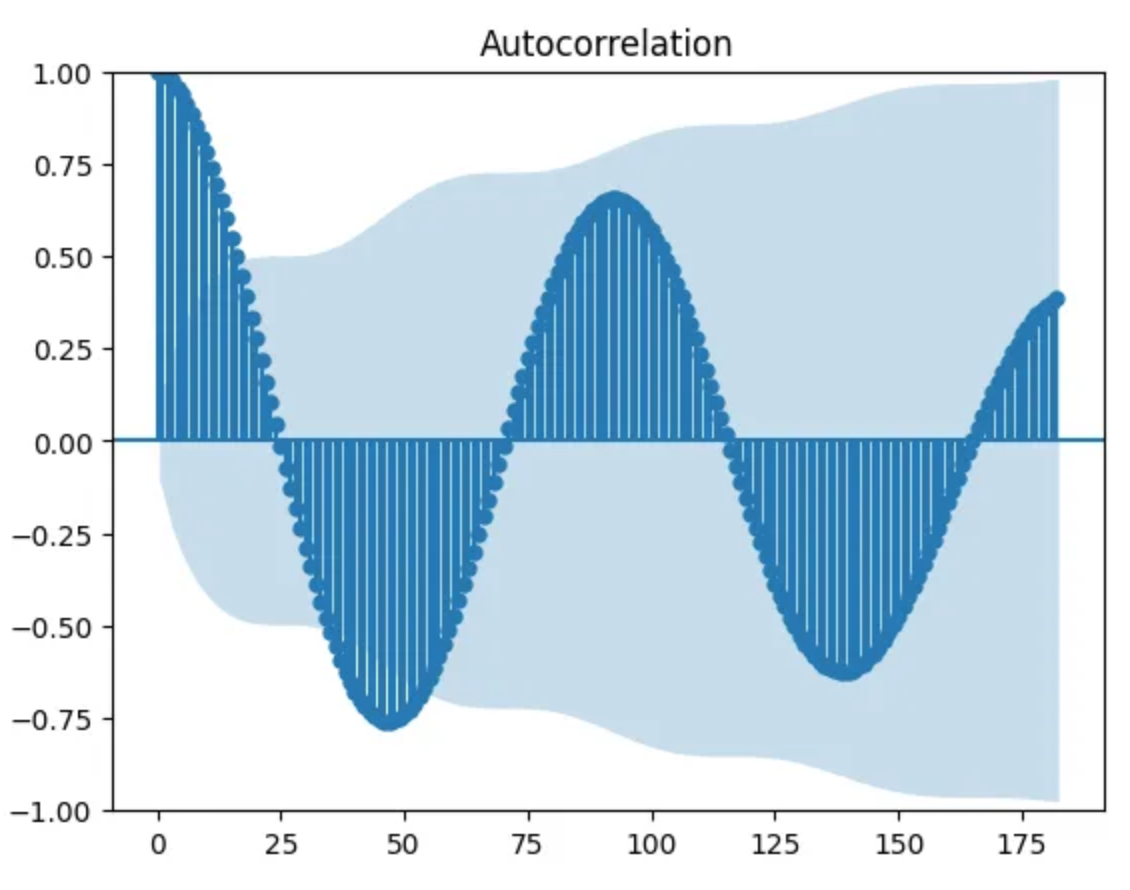
\includegraphics[width=\textwidth]{images/acs.png}
    \end{subfigure}
    \hfill
    \begin{subfigure}[t]{0.48\textwidth}
        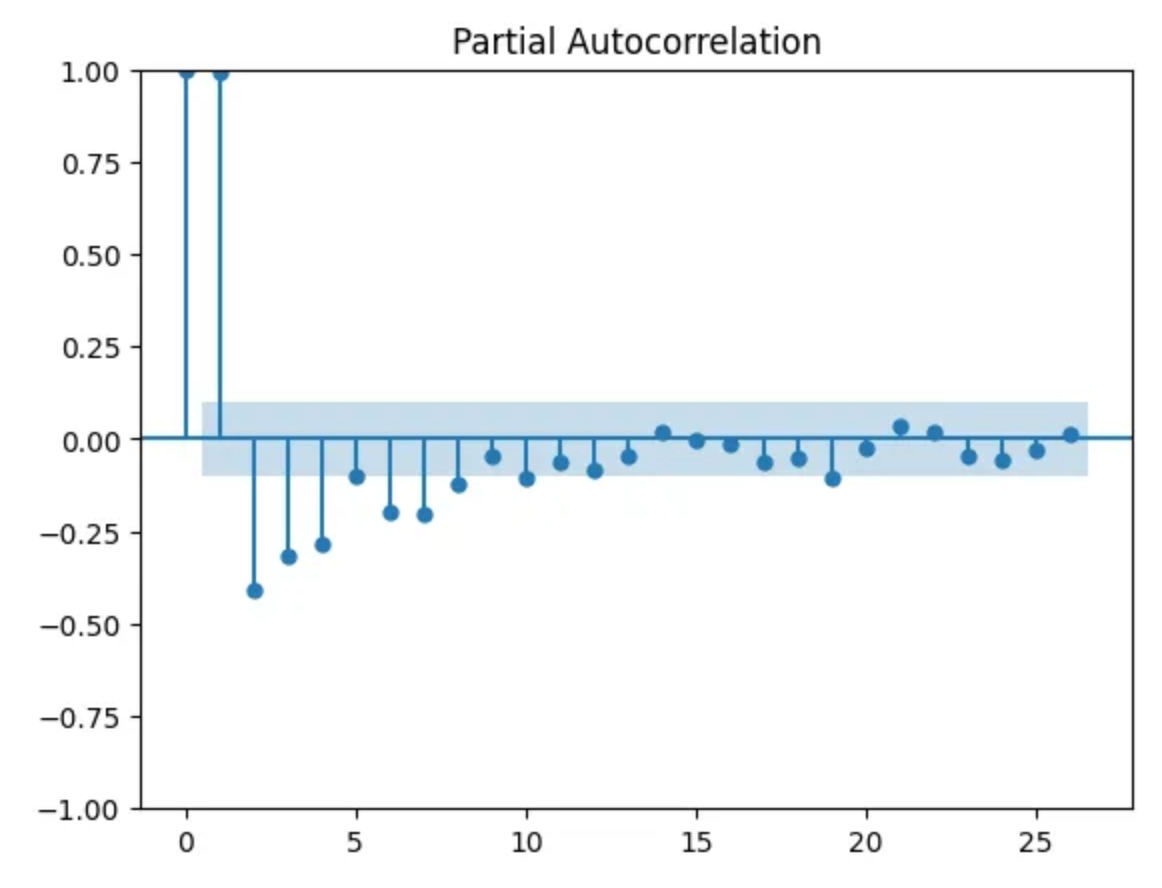
\includegraphics[width=\textwidth]{images/pacs.png}
    \end{subfigure}
    \caption{Autocorrelation (links) und Partial Autocorrelation (rechts)}
    \subcaption{\cite{kis2024}}
\end{figure}

Im ACF-Plot (links) erkennt man ein sinusoides Muster, was auf saisonale Zyklen hindeutet. Der PACF-Plot zeigt den sehr hohen Einfluss von lag 1, 2, 3, 4, 5, 7 und 8. Diese befinden sich ausserhalb des 95\% Konfidenzintervalls (blaues Band) und haben daher signifikanten Einfluss auf die gesamte Zeitreihe. \\
\\\textbf{Augmented Dickey-Fuller-Test (ADF):}\\
Statistisches Verfahren, das prüft, ob eine Zeitreihe eine Einheitswurzel enthält. Wenn eine Einheitswurzel-Charakteristik vorliegt wird ein Verschieben (lag) der Zeitreihe keine relevanten Informationen über die Prognose von $\hat{y_t}$ geben können. Wird eine Einheitswurzel gefunden liegt eine nicht-stationäre Zeitreihe vor. Wird im Gegenzug keine Einheitswurzel gefunden, kann von einer stationären Zeitreihe ausgegangen werden \cite{kwiatkowski1992}.\\
\\Das fertige ARIMA Modell wird also beschrieben mit den Parametern:
\begin{equation}
    ARIMA(p,d,q)
\end{equation}
Mit:
\begin{itemize}
    \item $p$: Ordnung der Autoregression (Wie viele vergangene Werte haben Einfluss auf den aktuellen Wert?)
    \item $q$: Ordnung des moving average (Wie viele vergangene Fehler werden haben Einfluss auf den aktuellen Wert?)
    \item $d$: Grad der Differenzierung bis die Zeitreihe stationär ist
\end{itemize}


\subsubsection{SARIMA}
ARIMA kann keine saisonalen Muster abbilden. Daher wird es zum \textbf{SARIMA-Modell} erweitert, indem es um die Parameter $(P, D, Q)_m$ ergänzt wird:
\begin{equation}
SARIMA(p,d,q)(P,D,Q)_m
\end{equation}
Hierbei beschreibt $m$ die saisonale Periodenlänge, z.\,B. $m=12$ für monatliche Daten mit jährlicher Saisonalität (vgl. \citeauthor{hyndman2018} \citeyear{hyndman2018}, Kap. 8.9).


\subsection{Bewertungsmetriken für Prognosegüte}
\label{subsec:metriken}

Zur Bewertung der Qualität von Vorhersagemodellen werden verschiedene statistische Fehlermaße verwendet. Die folgenden Metriken werden in dieser Arbeit zur Modellevaluation verwendet:

\paragraph{Mean Absolute Error (MAE):}
Der mittlere absolute Fehler gibt an, wie stark die Vorhersagewerte im Mittel von den tatsächlichen Werten abweichen \cite{vanderlei2020}:
\begin{equation}
\text{MAD} = \frac{1}{n} \sum_{t=1}^{n} |y_t - \hat{y}_t|
\end{equation}

\paragraph{Mean Absolute Percentage Error (MAPE):}
Die durchschnittliche prozentuale Abweichung des Fehlers von den jeweiligen tatsächlichen Werten \cite{vanderlei2020}.

\begin{equation}
\text{MAPE} = \frac{100}{n} \sum_{t=1}^{n} \left| \frac{y_t - \hat{y}_t}{y_t} \right|
\end{equation}

\paragraph{Root Mean Squared Error (RMSE):}
Die Wurzel des durchschnittlichen quadrierten Fehlers. Weniger anfällig für Ausreißer. Kann dank der Wurzel auch Modelle mit unterschiedlichen Skalen vergleichen.

\begin{equation}
\text{RMSE} = \sqrt{ \frac{1}{n} \sum_{t=1}^{n} (y_t - \hat{y}_t)^2 }
\end{equation}

Ein niedriger Wert dieser Metriken signalisiert eine hohe Prognosequalität. Die Auswahl geeigneter Metriken hängt dabei vom jeweiligen Anwendungsfall, der Skalierung der Daten und der Fehlertoleranz ab.

  \newpage

\section{Datengrundlage und Datenvorverarbeitung}
\label{sec:datengrundlage}

\subsection{Beschreibung des Datensatzes}
\label{subsec:datensatz}

Die Datengrundlage dieser Arbeit bildet der öffentlich verfügbare Datensatz \textit{Monthly and Annual Energy Consumption by Sector} der U.S. Energy Information Administration \citeyear{datensatz}. Der Datensatz umfasst den monatlichen Energieverbrauch der letzten Jahrzehnte in den Vereinigten Staaten, aufgeschlüsselt nach Verbrauchssektoren (Residential, Commercial, Industrial, Transportation) sowie aggregiert als \textit{Total Primary Energy Consumption}. Die Einträge reichen von Januar 1973 bis Dezember 2024 und bilden eine konsistente Zeitreihe zur Analyse des Energieverbrauchsverhaltens der US-Amerikaner.

\subsection{Datenvorverarbeitung}
\label{subsec:vorverarbeitung}

Für die Analyse wurde der Datensatz als CSV-Datei lokal gespeichert und verarbeitet. Die Zielvariable ist die Spalte \texttt{Total Primary Energy Consumption}, welche den monatlichen Gesamtverbrauch aller Sektoren aggregiert und als Primärenergie abbildet. Die folgenden Vorverarbeitungsschritte erfolgten mit Hilfe der Python-Bibliothek \textit{pandas}:

\begin{itemize}
    \item Die Zeitstempel aus der Spalte \texttt{Month} wurden in ein standardisiertes \texttt{datetime}-Format (\textit{YYYY-MM}) überführt und als Tabellenindex gesetzt
    \item Die Spalte \textit{Total Primary Energy Consumption} wurde extrahiert
    \item Dezimalzahlen der Spalte, die mit einem Komma (\texttt{,}) geschrieben waren, wurden zu einem Punkt (\texttt{.}) umgewandelt
    \item Möglicherweise fehlende Werte wurden durch lineare Interpolation eingefügt
    \item Abschließend wurde die Zeitreihe auf eine monatliche Frequenz - beginnend jeden Januar - standardisiert nach aufsteigendem Datum sortiert
\end{itemize}

Die vollständige Zeitreihe wurde zur Erstellung der Prognosemodelle in Trainings- und Testdaten aufgeteilt:

\begin{itemize}
    \item \textbf{Trainingsdaten:} Daten von Januar 1973 bis einschließlich Dezember 2014 (\texttt{TRAIN\_END\_YEAR = 2014})
    \item \textbf{Testdaten:} Daten von Januar 2015 bis einschließlich Dezember 2024 (\texttt{TEST\_END\_YEAR = 2024})
\end{itemize}

Diese Aufteilung orientiert sich an der best-practice ca. 20\% der Daten zur Modellvalidierung nach dem Training zu verwenden.


\subsection{Datenexploration}
\label{subsec:exploration}

Zur Untersuchung des Primärenergieverbrauchs in den Vereinigten Staaten wurde eine umfangreiche explorative Analyse durchgeführt. Diese soll grundlegende Strukturen, Trends und Muster in der Zeitreihe identifizieren und als Grundlage für die Modellierung dienen.

\subsubsection{Zeitlicher Verlauf}
\label{subsubsec:exploration-timeseries}

Die Zeitreihe (siehe Abbildung~\ref{fig:time_series}) zeigt einen übergeordneten, langfristigen Anstieg des Energieverbrauchs über die Jahrzehnte hinweg. Deutliche saisonale Schwankungen innerhalb der Jahre lassen auf zyklische Muster schließen, die v.a. durch Temperatur und Wirtschaftsaktivität beeinflusst sein dürften.

\begin{figure}[h!]
    \centering
    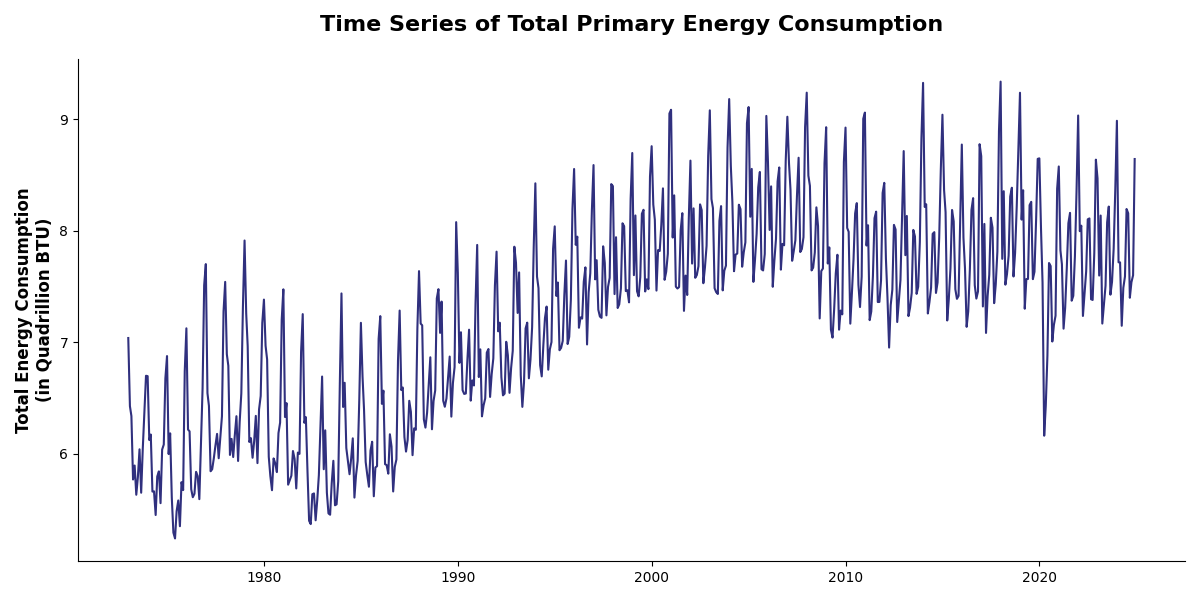
\includegraphics[width=0.9\textwidth]{images/expl/time_series.png}
    \caption{Zeitreihe des gesamten Primärenergieverbrauchs}
    \label{fig:time_series}
\end{figure}

\subsubsection{Gleitender Durchschnitt}
\label{subsubsec:exploration-moving-average}

Ein 12-monatiger gleitender Durchschnitt (Abbildung~\ref{fig:moving_average}) wurde berechnet, um kurzfristige Schwankungen zu glätten. Der geglättete Verlauf bestätigt einen strukturellen Aufwärtstrend mit Phasen moderater Stagnation, z.B. während wirtschaftlicher Krisen.

\begin{figure}[h!]
    \centering
    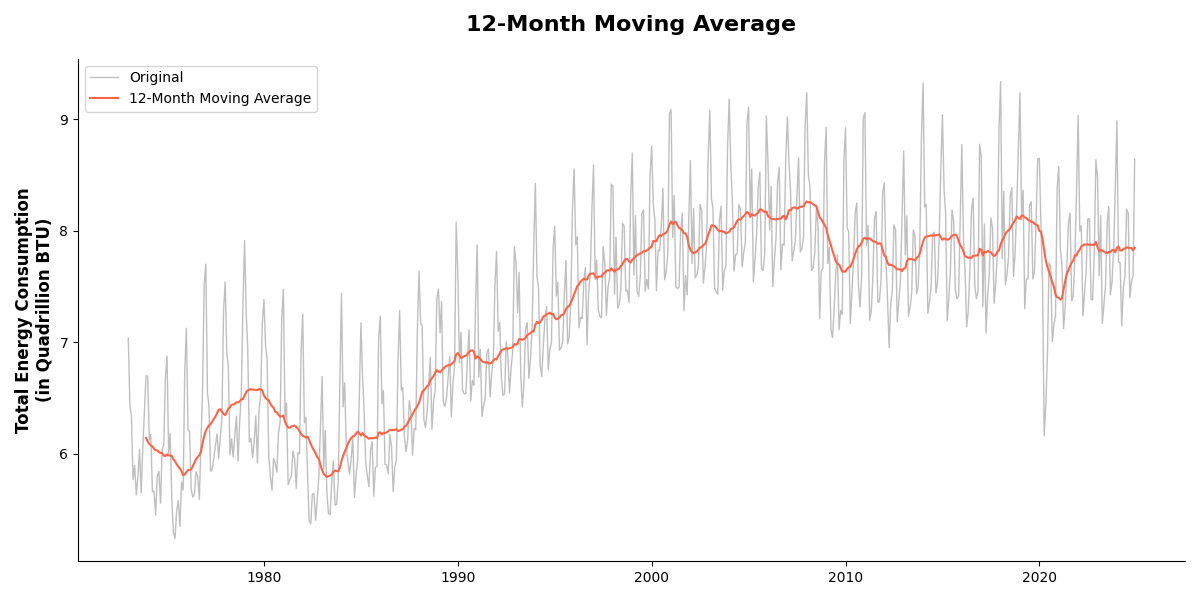
\includegraphics[width=0.9\textwidth]{images/expl/moving_average.png}
    \caption{12-Monats gleitender Durchschnitt des Energieverbrauchs}
    \label{fig:moving_average}
\end{figure}

\subsubsection{Saisonale Muster}
\label{subsubsec:exploration-seasonality}

Abbildung~\ref{fig:monthly_seasonality} zeigt den durchschnittlichen Verbrauch je Monat. Höhere Werte im Winter (Januar, Dezember) deuten auf Heizenergiebedarf hin, während die Sommermonate tendenziell niedrigere Verbräuche aufweisen.

\begin{figure}[h!]
    \centering
    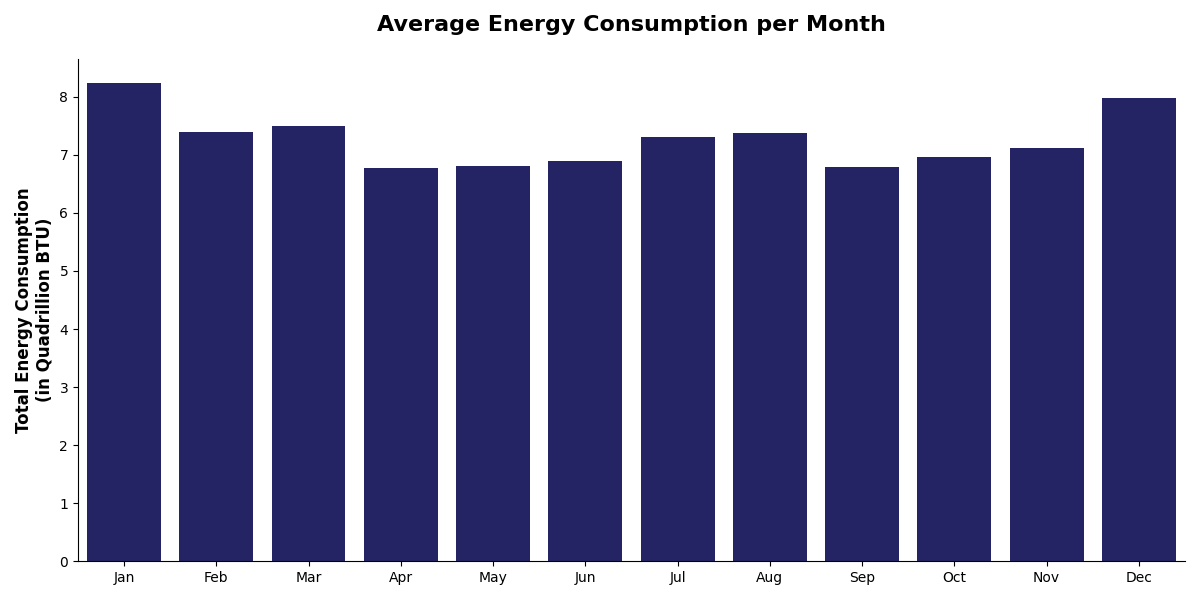
\includegraphics[width=0.9\textwidth]{images/expl/monthly_seasonality.png}
    \caption{Durchschnittlicher Energieverbrauch pro Monat}
    \label{fig:monthly_seasonality}
\end{figure}

Auch der Boxplot nach Monaten (Abbildung~\ref{fig:boxplot_by_month}) verdeutlicht die Streuung innerhalb der Monate und zeigt, dass insbesondere im Winter höhere und variablere Werte auftreten.

\begin{figure}[h!]
    \centering
    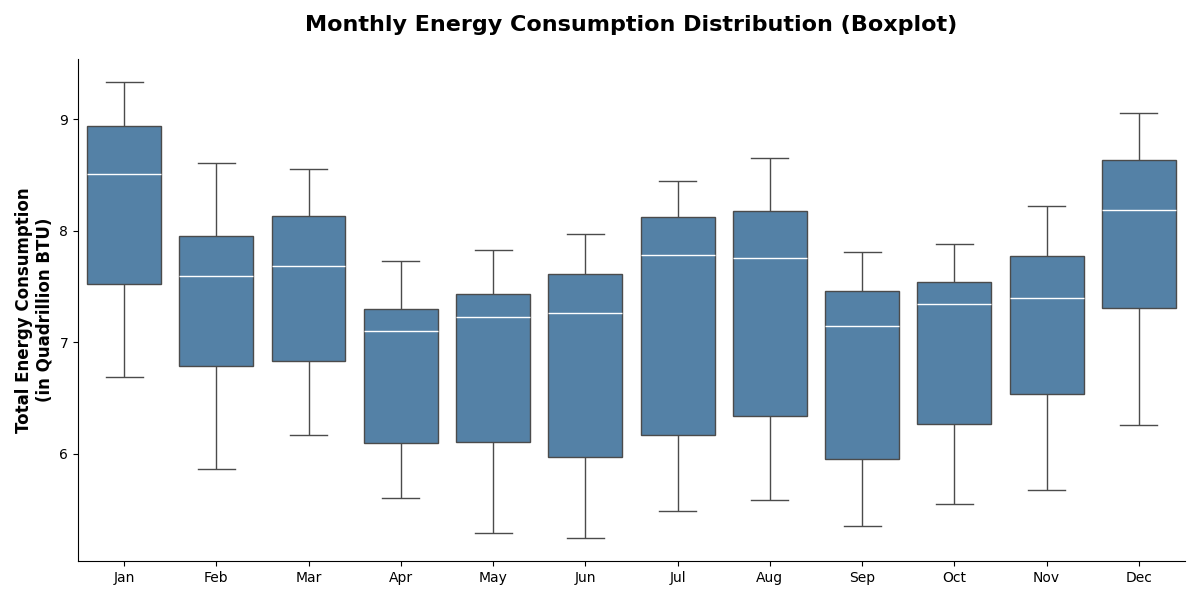
\includegraphics[width=0.9\textwidth]{images/expl/boxplot_by_month.png}
    \caption{Monatliche Verteilung des Energieverbrauchs (Boxplot)}
    \label{fig:boxplot_by_month}
\end{figure}

\subsubsection{Zerlegung der Zeitreihe}
\label{subsubsec:exploration-decomposition}

Eine additive Zerlegung (Abbildung~\ref{fig:decomposition}) teilt die Zeitreihe in Trend-, Saison- und Residualkomponenten. Die Saisonalität zeigt ein stark regelmäßiges Muster, während der Trend die langfristige Entwicklung nachzeichnet. Die Residuen erscheinen relativ zufällig verteilt.

\begin{figure}[h!]
    \centering
    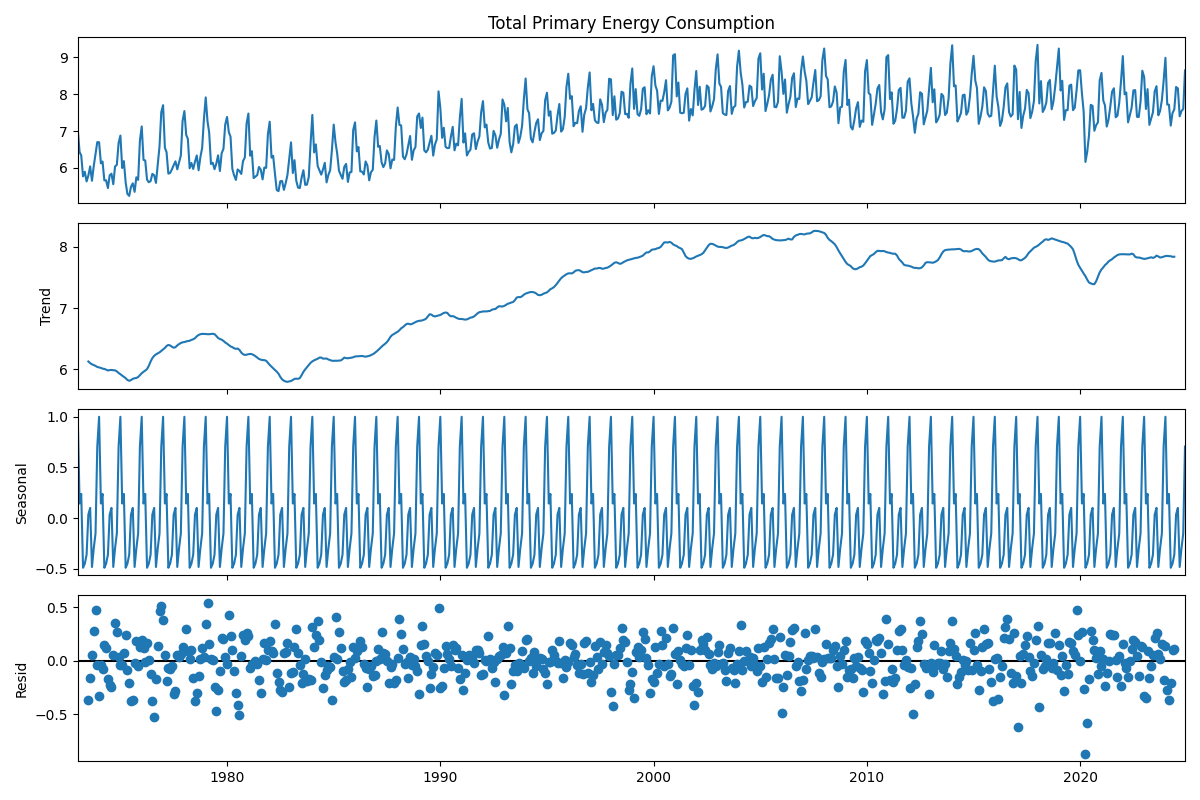
\includegraphics[width=0.95\textwidth]{images/expl/decomposition_additive.png}
    \caption{Additive Zeitreihen-Zerlegung}
    \label{fig:decomposition}
\end{figure}

\subsubsection{Verteilungsanalyse}
\label{subsubsec:exploration-distribution}

Das Histogramm (Abbildung~\ref{fig:histogram}) zeigt eine leicht rechtsschiefe Verteilung mit einer Häufung im Bereich 7–8 Quadrillion BTU. Extremwerte oberhalb von 9 deuten auf besonders verbrauchsintensive Phasen hin.

\begin{figure}[h!]
    \centering
    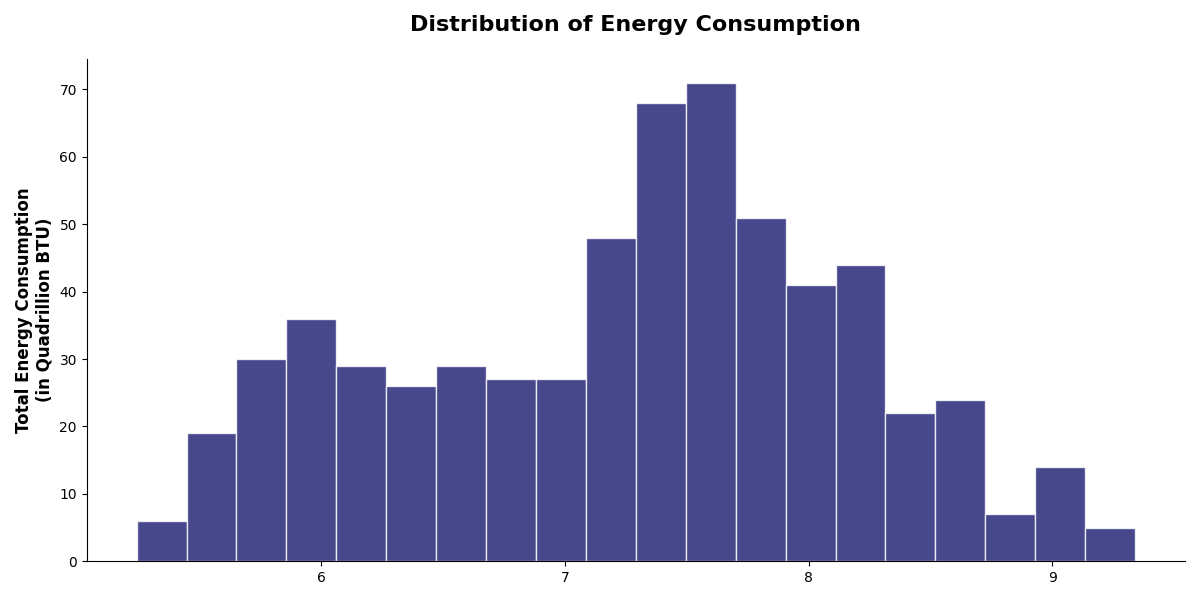
\includegraphics[width=0.9\textwidth]{images/expl/histogram.png}
    \caption{Verteilung des Energieverbrauchs}
    \label{fig:histogram}
\end{figure}

\subsubsection{Autokorrelation}
\label{subsubsec:exploration-acf}

Die Autokorrelationsanalyse (Abbildung~\ref{fig:acf_pacf}) zeigt signifikante Korrelationen über mehr als 36 Monate hinweg. Die PACF deutet auf eine autoregressive Struktur mit mehreren signifikanten Lags hin – u.a. bei Lag 1, 3, 6 und 12, was typische saisonale Muster bestätigt.

\begin{figure}[h!]
    \centering
    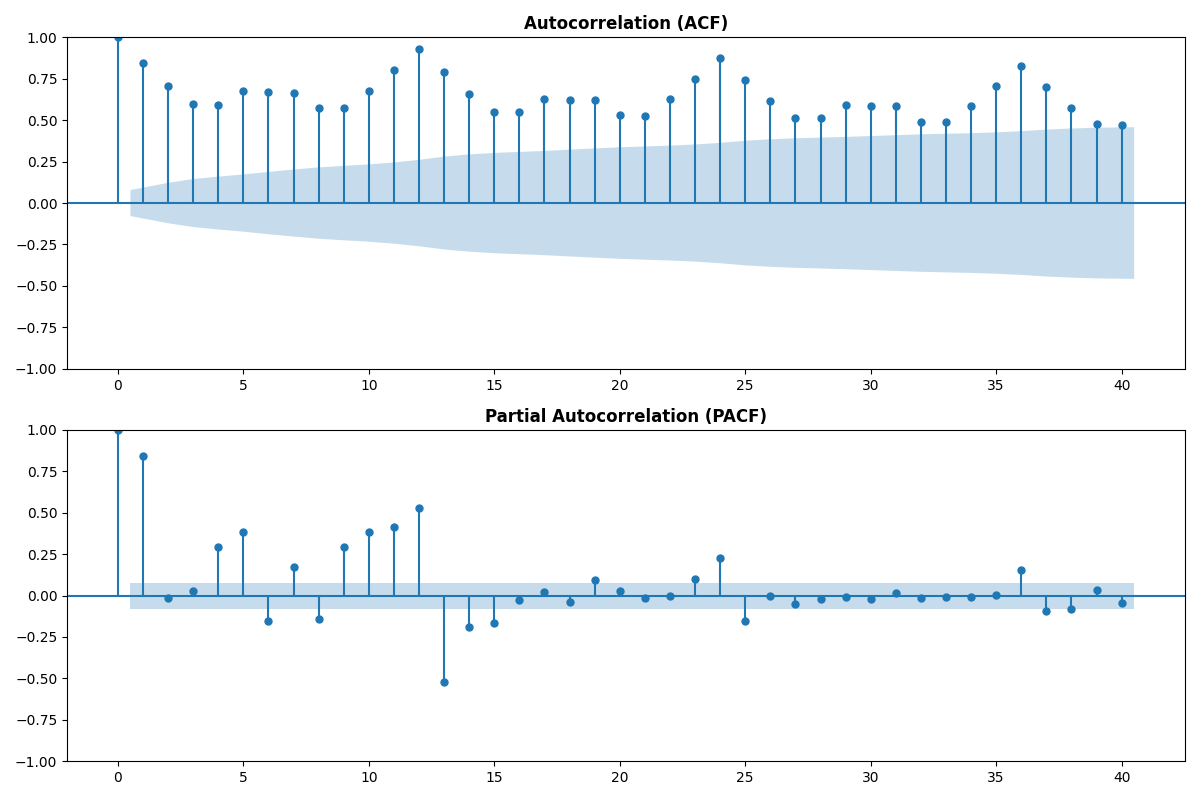
\includegraphics[width=0.95\textwidth]{images/expl/acf_pacf.png}
    \caption{Autokorrelation (ACF) und partielle Autokorrelation (PACF)}
    \label{fig:acf_pacf}
\end{figure}

  \newpage

\section{Methodik und Implementierung}
\label{sec:methodik}

\subsection{Überblick über den Modellierungsprozess}
\label{subsec:prozess}

\subsection{Umsetzung der Zeitreihenmodelle}
\label{subsec:umsetzung}

\subsubsection{Holt-Winters-Ansatz}
\label{subsubsec:holtwinters}

\subsubsection{ARIMA/SARIMA-Modell}
\label{subsubsec:arima-sarima}

\subsection{Modell-Validierung und Fehleranalyse}
\label{subsec:validierung}

\subsection{Implementierungsdetails}
\label{subsec:implementierung}
  \newpage

\section{Ergebnisse}
\label{sec:ergebnisse}

\subsection{Prognosegüte der Modelle im Gesamtvergleich}
\label{subsec:prognosevergleich}

\subsection{Visualisierung der Ergebnisse}
\label{subsec:visualisierung}

\subsection{Interpretation der Fehlerverteilung}
\label{subsec:fehlerinterpretation}
  \newpage

\section{Analyse von Ereigniseinflüssen (Event Impact Analysis)}
\label{sec:event-impact}

\subsection{Identifikation relevanter Ereignisse}
\label{subsec:ereignisse}

\subsection{Auswirkungen auf Prognosefehler}
\label{subsec:auswirkungen}

\subsection{Diskussion der Ursachen und Modellverhalten}
\label{subsec:diskussion-ereignisse}
  \newpage

\section{Interpretation der Ergebnisse}
\label{sec:interpretation}


\subsection{Qualität des Datensatzes}
\label{subsec:grenzen}

\subsection{Grenzen der gewählten Modelle}
\label{subsec:grenzen}

\subsection{Einfluss von externen Faktoren}
\label{subsec:einfluss}

\subsection{Möglichkeiten für Verbesserungen und Ausblick}
\label{subsec:ausblick}
  \newpage

\section{Fazit und Ausblick}
\label{sec:fazit}

\subsection{Zentrale Erkenntnisse}
\label{subsec:erkenntnisse}

\subsection{Relevanz für die Praxis}
\label{subsec:praxis}

\subsection{Potenziale für zukünftige Arbeiten}
\label{subsec:zukunft}

%%%%%%%%%%%%%%%%%%%%%%%%%%%%%%%%%%%%%%%%%%%%%%%%%%%%%%%%%%%%%
%%                                                         %%
%% /\   Bis hier die Änderungen zur Arbeit vornehmen    /\ %%
%%                                                         %%
%%%%%%%%%%%%%%%%%%%%%%%%%%%%%%%%%%%%%%%%%%%%%%%%%%%%%%%%%%%%%

	% Anhang
	% Tabellennummerierung mit Section
	\renewcommand{\thetable}{\Alph{section}.\arabic{table}}
	
	% Abbildungsnummerierung mit Section
	\renewcommand{\thefigure}{\Alph{section}.\arabic{figure}}

	% Listingsnummerierung mit Section
	\renewcommand{\thelstlisting}{\Alph{section}.\arabic{lstlisting}}
	
	% Abschluss
	\include{pages/18_literaturverzeichnis}
	\thispagestyle{empty}
\addcontentsline{toc}{section}{Selbständigkeitserklärung}
\begin{center}
    \vspace*{1cm}
    \Huge\bf Selbständigkeitserklärung\\
    \vspace*{2cm}
    \large\normalfont\singlespacing 
    Ich versichere hiermit, dass ich die vorliegende\\ \ifcase\myType Ausarbeitung \or Projektarbeit \or Bachelorarbeit \else Arbeit \fi mit dem Thema\\
    \vspace*{1cm}
    \Large\bf\myTopic\\
    \Large\normalfont\mySubTopic
    \vspace*{1cm}
    \large\normalfont
    \singlespacing 
    selbständig verfasst und keine anderen als die angegebenen\\Quellen und Hilfsmittel benutzt habe. Ich versichere zudem, 
    dass die eingereichte elektronische Fassung 
    mit der gedruckten Fassung übereinstimmt.\\
    \vfill
    \renewcommand{\arraystretch}{1.5} % Adjust spacing for the entire table
    \begin{tabularx}{\textwidth}{l@{\extracolsep\fill}r}
        % \rule{7cm}{0.3mm} 
        Ravensburg,
        & \rule{7.55cm}{0.3mm} \\[-0.2cm] % Name dicht unter Linie
        % Ort, Datum 
        den 20.06.2025
        & Fabian Bauriedl \\[0.7cm]
    \end{tabularx}
\end{center}

	
\end{document}

%%%%%%%%%%%%%%%%%%%%%%%%%%%%%%%%%%%%%%%%%%%%%%%%%%%%%%%%%%%%
%%                                                        %%
%% /\   /\  Ab hier keine Änderungen mehr vornehmen  /\   %%
%%                                                        %%
%%%%%%%%%%%%%%%%%%%%%%%%%%%%%%%%%%%%%%%%%%%%%%%%%%%%%%%%%%%%
